\documentclass[11pt,a4paper,oldfontcommands,oneside]{memoir}
\usepackage[utf8]{inputenc}
\usepackage{microtype}
\usepackage[dvips]{graphicx}
\usepackage{xcolor}
\usepackage{times}
\usepackage{graphicx}
\usepackage[spanish]{babel}
\usepackage[
breaklinks=true,colorlinks=true,
%linkcolor=blue,urlcolor=blue,citecolor=blue,% PDF VIEW
linkcolor=black,urlcolor=black,citecolor=black,% PRINT
bookmarks=true,bookmarksopenlevel=2]{hyperref}

\usepackage{geometry}
% PDF VIEW
% \geometry{total={210mm,297mm},
% left=25mm,right=25mm,%
% bindingoffset=0mm, top=25mm,bottom=25mm}
% PRINT
\geometry{total={210mm,297mm},
left=20mm,right=20mm,
bindingoffset=10mm, top=25mm,bottom=25mm}

\OnehalfSpacing
%\linespread{1.3}

%%% CHAPTER'S STYLE
\chapterstyle{bianchi}
%\chapterstyle{ger}
%\chapterstyle{madsen}
%\chapterstyle{ell}
%%% STYLE OF SECTIONS, SUBSECTIONS, AND SUBSUBSECTIONS
\setsecheadstyle{\Large\bfseries\sffamily\raggedright}
\setsubsecheadstyle{\large\bfseries\sffamily\raggedright}
\setsubsubsecheadstyle{\bfseries\sffamily\raggedright}


%%% STYLE OF PAGES NUMBERING
%\pagestyle{companion}\nouppercaseheads 
%\pagestyle{headings}
%\pagestyle{Ruled}
\pagestyle{plain}
\makepagestyle{plain}
\makeevenfoot{plain}{\thepage}{}{}
\makeoddfoot{plain}{}{}{\thepage}
\makeevenhead{plain}{}{}{}
\makeoddhead{plain}{}{}{}


\maxsecnumdepth{subsection} % chapters, sections, and subsections are numbered
\maxtocdepth{subsection} % chapters, sections, and subsections are in the Table of Contents


%%%---%%%---%%%---%%%---%%%---%%%---%%%---%%%---%%%---%%%---%%%---%%%---%%%

\begin{document}

%%%---%%%---%%%---%%%---%%%---%%%---%%%---%%%---%%%---%%%---%%%---%%%---%%%
%   TITLEPAGE
%
%   due to variety of titlepage schemes it is probably better to make titlepage manually
%
%%%---%%%---%%%---%%%---%%%---%%%---%%%---%%%---%%%---%%%---%%%---%%%---%%%
\thispagestyle{empty}

{%%%
\sffamily
\centering
\Large

~\vspace{\fill}

\includegraphics[scale=1]{logo.png} \\
{\huge 
\vspace{4cm}
INSTALACIÓN DE ROS, UBUNTU
}
\vspace{2.5cm}

{\LARGE
César Omar Alvarado Contreras \\
Jonathan Fonseca Camarena \\
Marcos Manzo Torres \\
Eduardo Robles Vázquez \\
Víctor Gabriel Tapia Casillas

}

\vspace{2.5cm}

Universidad Politécnica de la Zona Metropolitana de Guadalajara

\vspace{3.5cm}

Profesor: Carlos Enrique Morán Garabito

\vspace{\fill}

20 de septiembre del 2019

%%%
}%%%

\vspace{.5cm}
\hfill\break




\tableofcontents*

\clearpage

%%%---%%%---%%%---%%%---%%%---%%%---%%%---%%%---%%%---%%%---%%%---%%%---%%%
%%%---%%%---%%%---%%%---%%%---%%%---%%%---%%%---%%%---%%%---%%%---%%%---%%%

\chapter{Introducción}

ROS, es un conjunto de bibliotecas de software y herramientas que ayudan a crear aplicaciones roboticas. Desde controladores hasta algoritmos del estado del arte y con potentes herramientas de desarrollo, ROS tiene lo que necesitas para tu próximo proyecto de robótica. 

Entre sus fortalezas está que es usado en investigación, productos comerciales, educación y como centro de entretenimiento, tanto en el sector academico y el sector privado.

En este apartado, aprenderemos a realizar la instalación de ROS en el sistema operativo ubuntu, descargaremos las bibliotecas necesarias para el funcionamiento y creación de campo de trabajo en nuestra computadora. \cite{joseph2018kick}

\section{Preparación para instalación}
Primeramente como parte de la instalación, tenemos que configurar nuestro dispositivo para aceptar el software y todos los paquetes de ros.
\begin{figure}[h]
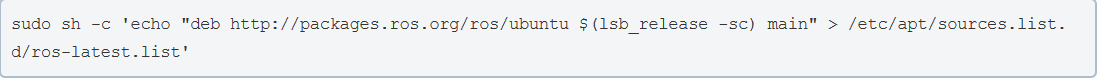
\includegraphics[scale=.8]{link1.png}
\end{figure}

Preparamos las llaves de nuestro sistema Ubuntu, como segunda parte del proceso
\begin{figure}[h]
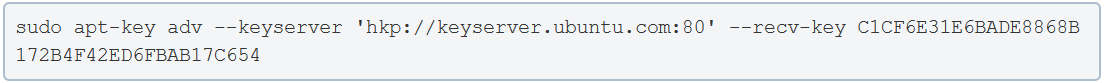
\includegraphics[scale=.8]{link11.png}
\end{figure}

\section{Instalación}
Procedemos a la instalación de ros, como primer paso nos aseguramos de que nuestro sistema Ubuntu se encuentra actualizado, para ello lanzamos el siguiente código.
\begin{figure}[h]
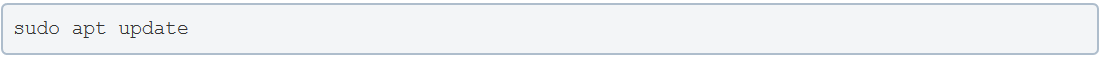
\includegraphics[scale=.8]{link20.png}
\end{figure}
Existen muchas herramientas diferentes en ROS. Se proporciona la configuración básica para que pueda comenzar. 
A continuación tenemos los elementos seleccionados y configuraciones recomendadas
Instalación completa en el escritorio: (recomendado) : ROS, rqt , rviz , bibliotecas genéricas de robots, simuladores 2D / 3D y percepción 2D / 3D

\begin{figure}[h]
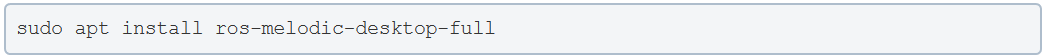
\includegraphics[scale=.8]{link13.png}
\end{figure}

Para encontrar paquetes disponibles después de realizar la instalación, usamos el siguiente código:

\begin{figure}[h]
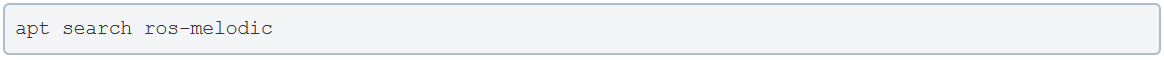
\includegraphics[scale=.8]{link15.png}
\end{figure}

Como siguiente paso instalamos rosdep para encontrar fácilmente las dependencias y componentes de ros.

\begin{figure}[h]
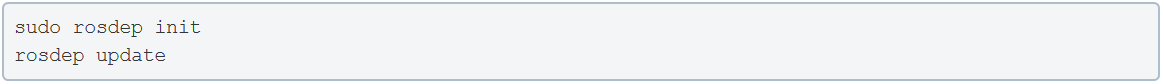
\includegraphics[scale=.8]{link16.png}
\end{figure}

\section{Declaración de entorno de trabajo}
Declaramos el archivo setup.bash
Si se tienen varias versiones de ros, se creará un conflicto con el archivo setup.bash, por lo que solo se recomienda una versión y una configuración del archivo setup.bash.
Después de esto, ya tenemos listo nuestro ambiente de trabajo. la instalación ha finalizado y solo falta realizar la comprobación de la correcta instalación.

\begin{figure}[h]
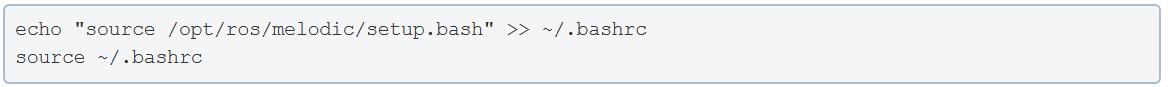
\includegraphics[scale=.8]{link17.png}
\end{figure}
\chapter{Comprobación de instalación}
En este apartado lanzeremos un código básico de ros, para comprobar que toda la instalación fue exitosa.
\section{Comprobación (roscore)}
Lanzamos el complemento roscore para verificar que la instalación se realizó con exito, nos aparecerá de la siguiente manera (si no se tuvo ningún error) como se puede observar en la figura \ref{roscore1}

\begin{figure}[h]
	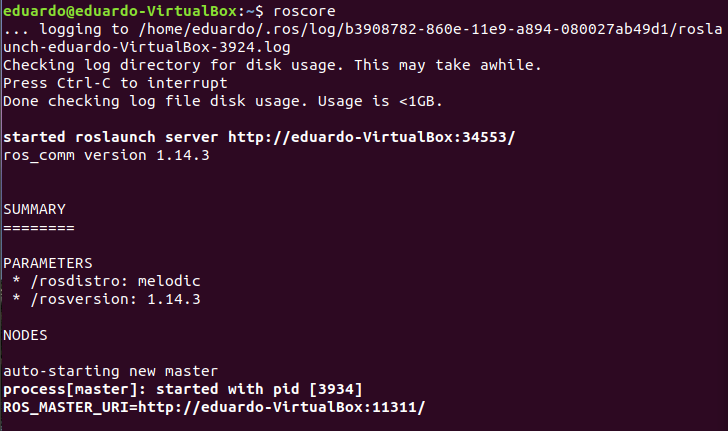
\includegraphics[scale=.75]{link21.png}
	\caption{Ejecución del comando roscore}
	\label{roscore1}
\end{figure}

\begin{figure}[h]
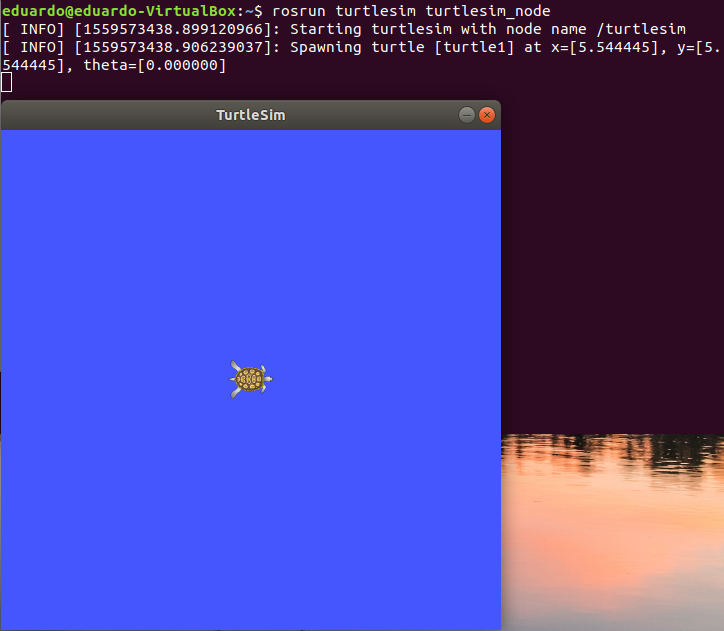
\includegraphics[scale=.75]{link23.png}
\caption{Ejecución de programa: turtlesim}
	\label{roscore2}
\end{figure}
\vspace{2cm}
\hfill

\chapter{Conclusión }
\section{Eduardo Robles Vázquez }
En esta práctica realizamos la instalación de Ros, cosa que ayudo a reafirmar nuestros conocimientos ya que en el cuatrimestre pasado habíamos instalado Ros y es posible que algunas cosas las recordáramos de manera diferente o las pasáramos por alto. En esta segunda ocasión el proceso de instalación fue más sencillo, demostrando así que la práctica hace al maestro. 

\vspace{2cm}
\hfill
\bibliographystyle{unsrt}
\bibliography{torres}


\end{document}

